\item \textbf{{[}DHS/PRELIM/9569/2021/P1/Q4{]} }
\begin{enumerate}
\item Explain how a linked list data structure could be more suitable than
an array data structure to implement a binary tree. \hfill{}{[}2{]}
\item (b) Suggest and justify one circumstance where an array structure
is more appropriate than a linked structure. \hfill{}{[}2{]}
\end{enumerate}
The diagram shows a binary tree before and after an inversion. 
\begin{center}
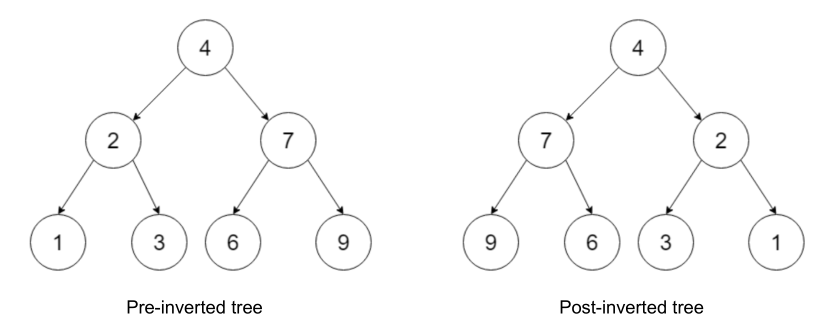
\includegraphics[width=0.5\paperwidth]{C:/Users/Admin/Desktop/Github/question_bank/static/img/9597-DHS-2021-P1-Q4-1}
\par\end{center}

Each node has these attributes: 
\begin{itemize}
\item \texttt{right} which is the pointer to right subtree 
\item \texttt{data} which is the value contained in each respective node
displayed above 
\item \texttt{left} which is the pointer to the left subtree
\end{itemize}
\begin{enumerate}
\item[(c)]  Write pseudocode for procedure \texttt{insert} which will add a
node to the post-inverted tree (which may be empty) in such a way
that if the new value of the node is \textbf{less} than the value
at the current node, the new node will be added to the \textbf{right}
subtree, or else it will be added to the left subtree. \texttt{insert}
takes in values \texttt{node\_data} and \texttt{root\_node} which
is the value to be added to the tree and the instance of the root
node of the tree respectively. \hfill{}{[}6{]}
\item[(d) ] A function \texttt{invertTree} takes in the root node of the above
pre-inverted tree, uses recursion to invert it into the post-inverted
tree, and returns the root node of the post-inverted tree. Write pseudocode
for the function and visualise it in a trace diagram. An incomplete
trace diagram is provided for you to begin with. Copy and complete
it. 
\noindent \begin{center}
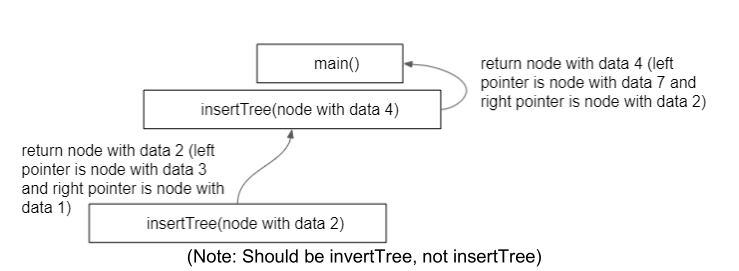
\includegraphics[width=0.5\paperwidth]{C:/Users/Admin/Desktop/Github/question_bank/static/img/9597-DHS-2021-P1-Q4-2}
\par\end{center}

(Note: Should be invertTree, not insertTree) \hfill{}{[}6{]}
\end{enumerate}